\subsection{Redes Neuronales Convolucionales}

Una Red Neuronal Convolucional (o CNN por sus siglas en inglés) es un tipo de red neuronal artificial en la cual las
neuronas procesan datos de entrada por medio de filtros de convolución. Esto implica el procesamiento de un grupo de
datos cercanos, lo que permite interpretar el contexto de un dato, en contraste con redes neuronales típicas. Esta
propiedad hace que las CNN sean el método preferido para el procesamiento de imágenes por medio de redes neuronales.
\autocite{hands-on-machine-learning} \autocite{ciresan-cnn}

Este método de procesamiento permite procesar una gran cantidad de entradas con una cantidad reducida de neuronas,
comparado con una red neuronal típica con la misma capacidad.

Por ejemplo, considerando una red neuronal con una capa de entrada y una capa siguiente con la misma cantidad de
neuronas $N$ en ambas, una red neuronal densa, es decir donde cada neurona de una capa está conectada a cada neurona de
la siguiente capa, contiene $N \times N$ conexiones. En contraste, una red neuronal convolucional equivalente estaría
compuesta de tan solo $N$ neuronas, mientras que al mismo tiempo captura un grupo de píxeles en cada neurona en lugar
de uno solo.

Para el procesamiento se utilizan los filtros de convolución, matrices de dimensiones reducidas comparadas con la
imagen, cuyas celdas contienen coeficientes. Este filtro se superpone sobre una sección de la imagen, y los valores de
los píxeles se multiplican con los de la celda superpuesta del filtro, y la suma de los productos es el resultado de la
convolución del grupo de píxeles. Con una representación adecuada de los datos de cada píxel, estos filtros, también
llamados {\it kernels }, pueden usarse en la detección de bordes en cualquier orientación, reducción de ruido,
aumentación de intensidad de píxeles de cierto color o brillo, entre otros. \autocite{ciresan-cnn}

\subsubsection{Aplicaciones}

CNN ya se han utilizado en todo tipo de aplicaciones relacionadas con imágenes y videos, entre ellas clasificación de
imágenes, segmentación de imágenes, detección de objetos e inclusive en análisis de imágenes de inundación para
predecir la gravedad de uno de estos tipos de desastre natural. \autocite{pally2022105285}

También se ha usado extensivamente en aplicaciones relacionadas a la teledetección, con una gran colección de técnicas,
conjuntos de datos, material de aprendizaje y software de libre acceso en artículos web, videos y repositorios de
código. \autocite{tds-landuse-classification} \autocite{repo-satellite-image-dl} Queda claro que los modelos
convolucionales son muy eficaces en el procesamiento de imágenes, y la cantidad de material estudiado relacionado a las
imágenes satelitales facilitaría enormemente la aplicación en el tema de este proyecto.

\subsubsection{Técnicas y arquitecturas}

Las primeras CNN surgieron en los años 90, con LeNet siendo la primera implementación que ganó atención. Esta red se
desarrolló para el reconocimiento de dígitos escritos a mano, y consistía de capas convolucionales, de {\it pooling},
el proceso de reducir la resolución y agrupar información de la capa anterior, y capas densamente, es decir
completamente, conectadas.

Recién en 2012 con AlexNet se logró el siguiente salto, con una competencia de reconocimiento visual. AlexNet se diseñó
con conjuntos de imágenes de gran escala en mente, compuesta de capas similares a LeNet, con algunas optimizaciones en
las funciones de activación y en medidas contra overfitting.

Nuevos desarrollos en los años siguientes se enfocaron en la optimización y la solución de problemas específicos.
VGGNet, originando en Oxford, se popularizó por su simplicidad, con kernels pequeños de 3x3 y capas convolucionales en
secuencias. Google introdujo GoogLeNet demostrando la efectividad del paralelismo con sus módulos {\it inception}, que
además mejoraron la capacidad de generalización usando kernels de diferentes tamaños al mismo tiempo. Otra
arquitectura, Redes Residuales o ResNets, abordaron el desafío de entrenar redes muy profundas por medio de conexiones
que saltan una o varias capas, facilitando el entrenamiento de redes de hasta cientas de capas. Otra red diseñada por
Google es MobileNet, una arquitectura diseñada para ejecutarse en ambientes de recursos limitados como dispositivos
móviles que busca equilibrar el rendimiento con la eficiencia.

Otra arquitectura importante es la U-Net, diseñada para la segmentación de imágenes biomédicas, que funciona mediante
reducciones sucesivas de resolución de la imagen de entrada, seguidas por aumentos sucesivos que se combinan con las
reducciones respectivas ya procesadas. Esta técnica permite entrenar modelos con mejor segmentación y menos datos de
entrenamiento, y con tarjetas gráficas modernas (de 2015 en adelante), procesar una imagen de $512 \times 512$ toma
menos de un segundo. \autocite{ronneberger2015unetconvolutionalnetworksbiomedical} También se han utilizado U-Nets en
aplicaciones de reducción de ruido en imágenes en modelos de difusión, lo cual se sigue utilizando en tecnologías de
generación de imágenes como {\it DALL-E}, {\it Midjourney} y {\it Stable Diffusion}. \autocite{ho2020denoising} También
se ha usado la arquitectura U-Net en segmentación de imágenes satelitales para identificar rasgos de imágenes, como
recursos de agua, bosques o agricultura con una intersección de entre 81 y 96\% con marcaciones manuales.
\autocite{khryashchev2018}

\begin{figure}
    \centering
    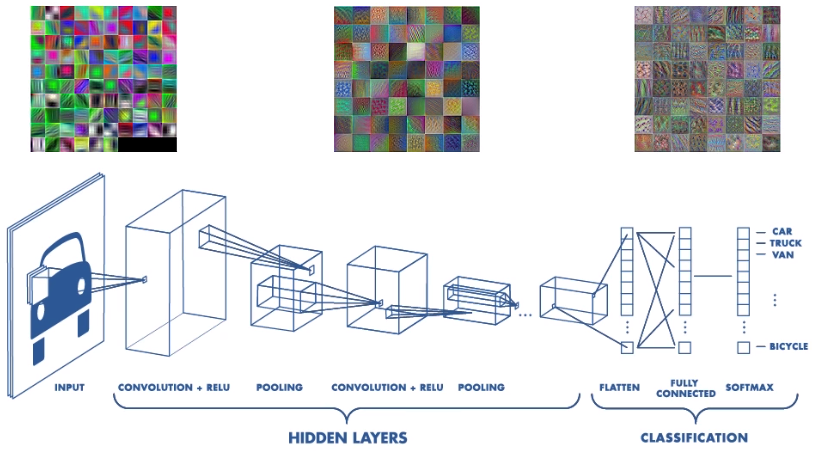
\includegraphics[width=0.6\textwidth]{img/cnn-figure.png}
    \caption{Ejemplo de red neuronal convolucional con varias capas de convolución y pooling, que preprocesan y
    comprimen la imagen, y varias capas convencionales, densamente conectadas, que hacen el trabajo de
    clasificación sobre un vector unidimensional.}
    \label{fig:2}
\end{figure}
